\documentclass{fefu}
\usepackage{float}
\usepackage{algorithm}
\usepackage{algpseudocode}
\usepackage{amsthm}
\usepackage{amsmath}
\usepackage{subcaption}
\usepackage[cache=false]{minted}
\newtheorem{definition}{Определение}
\newtheorem{lemma}{Лемма}
\author{Терехов Д.Е.}
\setschool{ШКОЛА ЕСТЕСТВЕННЫХ НАУК ДВФУ}
\setdepartment{кафедра информатики, математического и компьютерного моделирования}{Чеботарев}
\setgroup{Б8403а}
\renewcommand{\theenumi}{\Alph{enumi}}
\DeclareMathOperator{\sign}{sign}

\newenvironment{algo}[1][]
  {\begin{algorithm}[#1]
     \selectlanguage{english}
     \floatname{algorithm}{Алгоритм}
  }
  {\end{algorithm}}

\begin{document}
\tableofcontents
\pagebreak
\section*{Введение}
Преддипломная практика на кафедре информатики, математического и компьютерного моделирования – заключительные этап 
подготовки студента к презентации выпускной квалификационной работы. Актуальность преддипломной практики обусловлена 
необходимостью проведения итоговых вычислительных экспериментов, а также подготовке работы к внедрению на предприятии. 
Целью данной преддипломной практики являлось внедрение разработанных методов работы с триангуляцией множества вершин в 
игровой движок с открытым исходным кодом Citrus. Для достижения данной цели были поставлены следующие задачи:
\begin{itemize}
    \item Изучение архитектуры игрового движка с открытым исходным кодом Citrus;
    \item Перенос методов работы с триангуляцией множества вершин из тестового проекта в игровой движок Citrus;
    \item Совмещение функционала с результатами работы \cite{Gomenyuk};
    \item Тестирование;
    \item Написание отчета и документации. 
\end{itemize}
Содержание и программа практики:
\begin{itemize}
    \item Выполнение поставленных задач;
    \item Подведение итогов.
\end{itemize}
Период прохождения практики -- с 29 апреля 2019 года по 22 июня 2019 года. 
\subsection*{Описание предметной области}
\subsubsection*{Студия "Game Forest"}
Работа выполняется по заказу студии "Game Forest". "Game Forest" -- студия по разработке игр на мобильные устройства.
Наиболее успешные проекты:
\begin{itemize}
    \item 7 Wonders
    \item Gummy Drop
    \item Toy Story Drop
\end{itemize}

\subsubsection*{Citrus Game Engine}
Citrus -- игровой движок с открытым исходным кодом, распространяемый по лицензии GPL-3.0.
репозиторий размещен на платформе Github \cite{CitrusRepo}. Citrus Game Engine
состоит из следующих компонент:
\begin{itemize}
    \item Lime -- ядро игрового движка
    \item Lemon -- линкер сторонних библиотек
    \item Yuzu -- библиотека для сериализации
    \item Orange -- сборщик приложений
    \item Tangerine -- редактор сцен
    \item Kumquat -- генератор кода
\end{itemize}
\subsubsection*{Полигональный меш}
Полигональный меш (полигональная сетка) -- это совокупность вершин, рёбер и граней, которые определяют форму
многогранного объекта в трёхмерной компьютерной графике и объёмном моделировании. В двумерной компьютерной графике
меши используются для вершинной и скелетной анимации. Гранями меша обычно являются треугольники,
четырёхугольники или другие простые выпуклые многоугольники (полигоны), так как это упрощает рендеринг, но сетки могут
также состоять и из наиболее общих вогнутых многоугольников, или многоугольников с отверстиями.
\subsubsection*{PolygonMesh виджет}
В игровом движке Citrus существуют методы для работы с полигональным мешем --
DistortionMesh виджет. Проблема такого подхода заключается в неизменяемой структуре меша, которая является равномерной
сеткой $M\times N$, и в том, что каждая вершина сама по себе является узлом (Node) в иерархии объектов, что очень сильно
сказывается на производительности DistortionMesh. Были предложены следующие подходы к решению проблемы:
\begin{itemize}
    \item Попытаться оптимизировать текущую реализацию DistortionMesh;
    \item Избавиться от представления вершин в виде узлов в иерархии объектов;
    \item Создать новый виджет PolygonMesh, позволяющий задавать произвольное положение вершин, а также не имеющий
    представление вершин в виде узлов иерархии объектов.
\end{itemize}
Было принято решение разработать новый виджет PolygonMesh. Для того чтобы вершины могли
иметь не предопределённые позиции, необходимо поддерживать специальную структуру представляющую собой
триангуляцию множества точек, что является моей частью работы по созданию PolygonMesh виджета. Были выдвинуты
следующие требования к методам триангуляции множества точек:
\begin{itemize}
    \item Алгоритм триангуляции должен быть online;
    \item Алгоритм триангуляции должен быть достаточно быстрым, чтобы использовать его в редакторе сцен
    Tangerine для нового виджета PolygonMesh.
\end{itemize}
Разработанные методы триангуляции используются в работе \cite{Gomenyuk}.
\section{Математические методы}
\subsection{Триангуляция Делоне}
Среди возможных триангуляций множества точек своими свойствами выделяется триангуляция Делоне. Триангуляция Делоне
минимизирует максимальный угол, двойственна диаграмме Вороного, существуют online и offline алгоритмы построения
триангуляции Делоне трудоемкостью $O(n\log{}n)$ в худшем и среднем случаях. Кроме того, известны алгоритмы, позволяющие
в ряде случаев достичь в среднем $O(n)$. В триангуляции Делоне есть ряд недостатков: возможны образования плохих
треугольников, граница области может не проявится в триангуляции. Для обоих проблем есть пути решения: алгоритмы
уточнения Делоне \cite{DelaunayRefinement} и триангуляция Делоне с ограничениями соответственно.
\begin{definition}
    \textit{Триангуляция Делоне} $D$ это граф над множеством вершин $V$. Любая окружность на плоскости
    называется \textit{пустой}, если она не содержит в себе ни одной вершины из $V$. Пусть $u$ и $v$ любые 2 вершины из
    $V$. Ребро $uv$ принадлежит $D$ тогда и только тогда, когда существует пустая окружность, проходящая через вершины
    $u$ и $v$. Ребро, удовлетворяющее этому свойству, называется ребром Делоне.
\end{definition}
Триангуляция Делона множества вершин уникальна, поскольку приведенное выше определение точно устанавливает однозначный
тест на наличие или отсутствие ребра в триангуляции.
Совершенно не очевидно, что множество ребер Делоне в совокупности образует триангуляцию. Для определения
выше триангуляция Делоне гарантированно будет триангуляцией, только если ни одна из четверки вершин $V$ не лежит на одной
окружности. Дадим понятие треугольника Делоне.
\begin{definition}
    Треугольник называется треугольником Делоне, если окружность, описанная вокруг треугольника пуста.
\end{definition}
\begin{lemma}
    Пусть $T$ -- триангуляция. Если все треугольники $T$ являются треугольниками Делоне, то все ребра $T$ являются
    ребрами Делоне. И наоборот.
\end{lemma}
\begin{proof}
    Если все треугольники из $T$ Делоне, то окружность, описанная вокруг треугольника, пуста. Так как любое ребро
    из $T$ принадлежит треугольнику из $T$, то любое ребро содержится в пустой окружности, а значит оно Делоне.
\end{proof}
\begin{definition}
    Ребро является ребром Делоне локально, если оно является ребром Делоне, учитывая только пару треугольников, для
    которых это ребро общее.
\end{definition}
\begin{figure}[H]
    \centering
    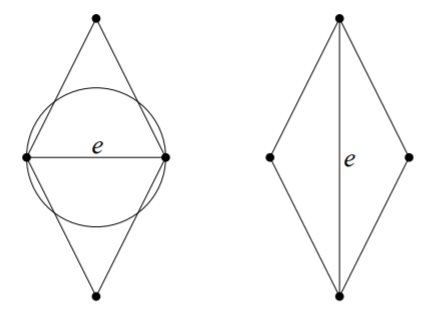
\includegraphics{images/Flip.jpg}
    \caption{Флип ребра}
\end{figure}
Четырехугольник можно триангулировать двумя способами. Назовем флипом смену триангуляции четырехугольника (рис. 4).

\begin{figure}[H]
    \centering
    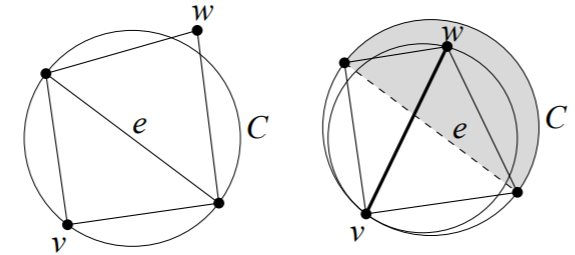
\includegraphics{images/FlipLemma.jpg}
    \caption{Слева - $e$ ребро Делоне локально, справа -- флип ребра $e$ образует ребро, которое является ребром Делоне
    локально}
\end{figure}
\begin{lemma}
    Пусть $e$ ребро триангуляции $T$. Либо $e$ ребро Делоне локально, либо его можно флипнуть, и полученное ребро будет
    ребром Делоне локально.
\end{lemma}
\begin{proof}
    Пусть $v$ и $w$ вершины, противолежащие $e$, которые вместе с $e$ определяют четырехугольник. Пусть $C$ окружность
    проведенная через $v$ и концы $e$. Либо $w$ строго внутри, либо на окружности, либо снаружи.

    Если $w$ лежит на окружности либо снаружи, то $e$ Делоне локально.

    Если $w$ лежит внутри $C$, то четырехугольник строго выпуклый. Значит $e$ возможно флипнуть. Кроме того окружность,
    проведенная через $v$ и $w$ касается $C$ в вершине $v$ и не содержит концов $e$. Значит ребро $vw$ Делоне локально.
\end{proof}
\subsubsection{Способы проверки свойства Делоне}
\paragraph{Проверка через уравнение описанной окружности}
Уравнение окружности, проходящей через точки $(x_1, y_1), (x_2, y_2), (x_3, y_3)$, можно записать в виде:
\[
    \left|\begin{matrix}
        x^2 + y^2 & x & y & 1\\
        x^2_1 + y^2_1 & x_1 & y_1 & 1\\
        x^2_2 + y^2_2 & x_2 & y_2 & 1\\
        x^2_3 + y^2_3 & x_3 & y_3 & 1
    \end{matrix}\right| = 0
\]
или же как $(x^2 + y^2)\cdot a - x \cdot b + y \cdot c - d = 0$, где
\[
    a = \left|\begin{matrix}
        x_1 & y_1 & 1\\
        x_2 & y_2 & 1\\
        x_3 & y_3 & 1
    \end{matrix}\right|,
    b = \left|\begin{matrix}
        x^2_1 + y^2_1 & y_1 & 1\\
        x^2_2 + y^2_2 & y_2 & 1\\
        x^2_3 + y^2_3 & y_3 & 1
    \end{matrix}\right|,
    c = \left|\begin{matrix}
        x^2_1 + y^2_1 & x_1 & 1\\
        x^2_2 + y^2_2 & x_2 & 1\\
        x^2_3 + y^2_3 & x_3 & 1
    \end{matrix}\right|,
    d = \left|\begin{matrix}
        x^2_1 + y^2_1 & y_1 & y_1\\
        x^2_2 + y^2_2 & y_2 & y_2\\
        x^2_3 + y^2_3 & y_3 & y_3
    \end{matrix}\right|
\]

Тогда условие Делоне для любого заданного треугольника будет
выполняться тогда и только тогда, когда для любого узла $(x_0, y_0)$ триангуляции будет $\left(a \cdot (x^2_0 + y^2_0) -
b\cdot x_0 + c \cdot y_0 - d\right)\cdot \sign a \geq 0$. Для упрощения вычислений можно заметить, что если тройка
точек $(x_1, y_1), (x_2, y_2), (x_3, y_3)$ является правой, то всегда $\sign a = -1$, если всегда левой, то $\sign a = 1$.

Непосредственная реализация такой процедуры проверки требует 29 умножений, а также 24 операций  сложения и вычитания.
\paragraph{Проверка суммы противолежащих углов}
Свойство Делоне для данного треугольника $\Delta \left((x_1, y_1), (x_2, y_2), (x_3, y_3)\right)$ будет выполнятся
только тогда, когда для любой другой точки $(x_0, y_0)$ триангуляции $\alpha + \beta \leq \pi$ (рис. 6). Это условие
эквивалентно $\sin\left(\alpha + \beta\right) \geq 0$, т.е.
\[
    \sin\alpha \cdot \cos\beta + \cos\alpha \cdot \sin\beta \geq 0
\]

Значение синусов и косинусов углов можно вычислить по следующим формулам:
\[
    \begin{matrix}
        \cos\alpha = \frac{(x_0 - x_1)\cdot(x_0 - x_3) + (y_0 - y_1)\cdot(y_0 - y_3)}{\sqrt{(x_0 - x_1)^2 + (y_0 - y_1)^2}
    \sqrt{(x_0 - x_3)^2 + (y_0 - y_3)^2}},\\
    \cos\beta = \frac{(x_2 - x_1)\cdot(x_2 - x_3) + (y_2 - y_1)\cdot(y_2 - y_3)}{\sqrt{(x_2 - x_1)^2 + (y_2 - y_1)^2}
    \sqrt{(x_2 - x_3)^2 + (y_2 - y_3)^2}},\\
    \sin\alpha = \frac{(x_0 - x_1)\cdot(y_0 - y_3) + (x_0 - x_3)\cdot(y_0 - y_1)}{\sqrt{(x_0 - x_1)^2 + (y_0 - y_1)^2}
    \sqrt{(x_0 - x_3)^2 + (y_0 - y_3)^2}},\\
    \sin\beta = \frac{(x_2 - x_1)\cdot(y_2 - y_3) + (x_2 - x_3)\cdot(y_2 - y_1)}{\sqrt{(x_2 - x_1)^2 + (y_2 - y_1)^2}
    \sqrt{(x_2 - x_3)^2 + (y_2 - y_3)^2}}
    \end{matrix}
\]

Подставив значения в формулу, получим следующую формулу проверки:
\small
\begin{equation*}
    \begin{split}
        & \left((x_0 - x_1)(y_0 - y_3) - (x_0 - x_3)(y_0 - y_1)\right)\cdot \left((x_2 - x_1)(x_2 - x_3) + (y_2 - y_1)(y_2 - y_3) \right) + \\
        & + \left((x_0 - x_1)(x_0 - x_3) + (y_0 - y_1)(y_0 - y_3)\right)\cdot \left((x_2 - x_1)(y_2 - y_3) - (x_2-x_3)(y_2 - y_1)\right)\geq 0
    \end{split}
\end{equation*}
\normalsize
Непосредственная реализация такой процедуры требует 10 операций умножения, а также 13 операций сложения и вычитания.
\begin{figure}[H]
    \centering
    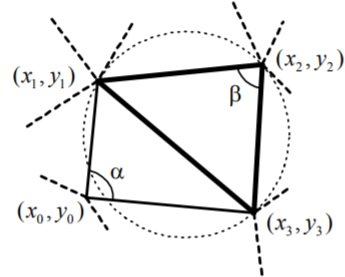
\includegraphics{images/OppositeAngles.jpg}
    \caption{Проверка суммы противолежащих углов}
\end{figure}
\paragraph{Модифицированная проверка суммы противолежащих углов}
В \cite{ModifiedOppositeAngles} предложено вычислять не сразу все скалярные и векторные произведения. Вначале нужно
вычислить только часть выражения, соответствующую $\cos \alpha$ и $\cos \beta$:
\begin{equation*}
    \begin{split}
        s_\alpha = (x_0 - x_1)(x_0 - x_3) + (y_0 - y_1)(y_0 - y_3),\\
        s_\beta = (x_2 - x_1)(x_2 - x_3) + (y_2 - y_1)(y_2 - y_3).
    \end{split}
\end{equation*}

Тогда, если $s_\alpha < 0$ и $s_\beta < 0$, то $\alpha > 90^\circ, \beta > 90^\circ$, и поэтому Делоне не выполняется.
Если $s_\alpha \geq 0$ и $s_\beta \geq 0$, то $\alpha \leq 90^\circ, \beta \leq 90^\circ$, и поэтому Делоне выполняется.
Иначе требуются полные вычисления по формуле.

Такое усовершенствование позволяет в среднем на 20-40\% сократить количество выполняемых арифметических операций (
примерно до 7 умножений, а также 9 сложений и вычитаний). Дополнительным преимуществом это проверки перед предыдущим
способом является большая устойчивость к потере точности в промежуточных вычислениях с использованием вещественной
арифметики с плавающей точкой.
\begin{table}[H]
    \centering
    \begin{center}
        \begin{tabular} { |c|c|c| }
            \hline
            Способ проверки & Число $\times$ и $\div$ & Число $+$ и $-$\\ [0.5ex]
            \hline
            Уравнение описанной окружности & 29 & 24\\
            Сумма противолежащих углов & 10 & 13\\
            Модифицированная сумма противолежащих углов & \textasciitilde 7 & \textasciitilde 9\\
            \hline
        \end{tabular}
    \end{center}
\end{table}
\subsubsection{Структуры для представления триангуляции}
\paragraph{Triangle}
\begin{figure}[H]
    \centering
    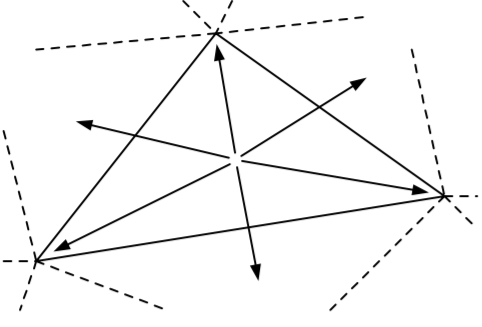
\includegraphics{images/TriangleStructure.png}
    \caption{Triangle}
\end{figure}
Jonathan Richard Shewchuk в своей работе \cite{MeshGeneration} предложил использовать структуру данных вместо
quade-edge, разработанной Guibas и Stolfi\cite{QuadEdge}, в явном виде
представляющую треугольник. Структура содержит в себе массив из 3 вершинных индексов, массив указателей на соседние
треугольники, где $i$-ый треугольник имеет общее ребро, лежащее напротив $i$ вершины, с текущим треугольником, а также
массив ориентаций, где $i$ элемент показывает, что текущий треугольник имеет индекс $orientations[i]$ в $i$ соседнем
треугольнике. Массив $orientations$ можно опустить и хранить данную информацию в указателях на соседние треугольники.

\begin{table}[H]
    \centering
    \begin{tabular}{|c|c|c|}
        \hline
        Vertices & Целочисленный массив & Индексы вершин\\
        Triangles & Массив указателей на Triangle & Смежные треугольники\\
        \hline
    \end{tabular}
    \caption{Структура Triangle}
\end{table}

Данная структура данных более экономна по занимаемому месту. Алгоритмы триангуляции имеют меньшую константу (примерно в
2 раза) при реализации с использованием данной структуры по сравнению с quade-edge.
\paragraph{HalfEdge}
Структура HalfEdge представляет собой ориентированное ребро, которое имеет индекс начала ребра, указатель на следующее
ребро и на ребро-близнец, направленное в обратную сторону. Недостатками данной структуры является представление
треугольников в неявном виде, а также большой расход памяти.

\begin{table}[H]
    \centering
    \begin{tabular}{|c|c|c|}
        \hline
        Origin & Целочисленный & Индекс вершины начала ребра\\
        Next & Указатель на HalfEdge & Следующее ребро \\
        Twin & Указатель на HalfEdge & Ребро-близнец \\
        \hline
    \end{tabular}
    \caption{Структура HalfEdge}
\end{table}
\paragraph{CompactHalfEdge}

Существует компактное представление для HalfEdge\cite{CHE}:

\begin{table}[H]
    \centering
    \begin{tabular}{|c|c|p{6cm}|}
        \hline
        Vertices & Массив Vertex & Вершины меша\\
        \hline
        Origins & Целочисленный массив & $i$ элемент -- индексы вершины начала $i$ ребра\\
        \hline
        Twins & Целочисленный массив & $i$ элемент -- индекс ребра-близнеца для $i$ ребра\\
        \hline
        VerteciesIncidentEdge & Целочисленный массив & $i$ элемент -- индекс какого-либо ребра, инцидентного $i$ вершине\\
        \hline
        EdgeMap & Целочисленный массив & Массив ребер, задающих треугольники; каждый треугольник должен входить единожды\\
        \hline
    \end{tabular}
    \caption{Структура CompactHalfEdge}
\end{table}

В данной работе используется модифицированное представление Compact-\\HalfEdge:
\begin{table}[H]
    \centering
    \begin{tabular}{|c|c|c|}
        \hline
        Vertices & Массив Vertex & Вершины меша\\
        \hline
        HalfEdges & Массив HalfEdge & Ребра меша\\
        \hline
    \end{tabular}
    \caption{Модифицированная структура CompactHalfEdge}
\end{table}

Где HalfEdge:

\begin{table}[H]
    \centering
    \begin{tabular}{|c|c|c|}
        \hline
        \multicolumn{3}{ |c| }{HalfEdge}\\
        \hline
        \hline
        Origin & Целочисленный & Индекс вершины начала ребра\\
        Next & Целочисленный & Индекс следующего ребра \\
        Twin & Целочисленный & Индекс ребра-близнеца \\
        \hline
    \end{tabular}
    \caption{Структура HalfEdge}
\end{table}

\subsubsection{Итеративный алгоритм построения триангуляции Делоне}
В настоящее время известно большое множество различных алгоритмов построения триангуляции Делоне. Многие из них описаны
в \cite{Skvorcov}. Формально любой итеративный алгоритм выглядит так:
\begin{itemize}
    \item Примитивные случаи обрабатываются отдельно (случай 1, 2 и 3 вершин).
    \item Далее для каждой точки повторяются следующие операции
    \begin{enumerate}
        \item Происходит локализация вершины, т.е. находится треугольник, в который попадает вершина. Если вершина не попадает
        в текущую триангуляцию, то она добавляется особым способом (п. \ref{AddOutsideOfTriangulationVertex}).
        \item Происходит построение новых треугольников.
        \item Проводятся локальные проверки построенных треугольников на выполнению свойства Делоне и выполняются
        необходимые перестроения.
    \end{enumerate}
\end{itemize}
Сложность итеративного алгоритма складывается из трудоемкости поиска треугольника, в который попадает новая вершина,
трудоемкости построения новых треугольников и проверок свойства Делоне с дальнейшим перестроением пар соседних
треугольников, не удовлетворяющих свойству Делоне. За все шаги алгоритма будет добавлено не более $3 \cdot n$
треугольников, где $n$ - общее число вершин. Поэтому общее время работы алгоритма составляет $O(n)$. Любое добавление
новой вершины в триангуляцию может нарушить условия Делоне, поэтому после добавления вершины производится локальная
проверка триангуляции на условие Делоне всех построенных треугольников, что может привести к перестроению всей
триангуляции в худшем случае. Поэтому трудоемкость перестроений составляет $O(n)$. Однако среднее число таких перестроений
на реальных данных составляет не более 3\cite{Skvorcov2}. Таким образом, наибольший вклад в трудоемкость итеративного
алгоритма дает процедура локализации точки. Это то, чем в основ отличаются все итеративные алгоритмы построения
триангуляции Делоне.

Итеративные алгоритмы можно разделить на группы по методы локализации вершины:
\begin{itemize}
    \item Простые итеративные алгоритмы
    \item Алгоритмы с индексированием поиска треугольников
    \item Алгоритмы с кэшированием поиска треугольников
    \item Итеративные алгоритмы триангуляции с измененным порядком добавления точек
\end{itemize}
 Итеративные алгоритмы триангуляции с измененным порядком добавления точек не подходят для поставленной задачи, так как
 множество вершин заранее не известно. Алгоритмы с индексированием и кэшированием поиска треугольников не подходят, по
 причине того что поставленная задача создает большие накладные расходы на поддержание структуры данных.

 Рассмотрим варианты локализации треугольника для простого итеративного алгоритма:
\begin{figure}[H]
    \centering
    \begin{subfigure}[t]{.3\linewidth}
    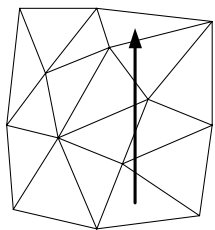
\includegraphics[scale=0.8]{images/ThrougSegmentIntersection.jpg}
        \caption{Переход вдоль прямой}
        \label{LineThrough}
    \end{subfigure}
    \begin{subfigure}[t]{.3\linewidth}
    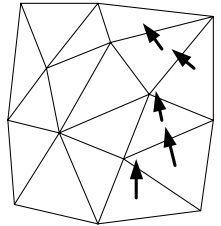
\includegraphics[scale=0.8]{images/ClosestEdge.jpg}
        \caption{Переход через ближайшее к цели ребро}
        \label{ClosestEdge}
    \end{subfigure}
    \begin{subfigure}[t]{.3\linewidth}
    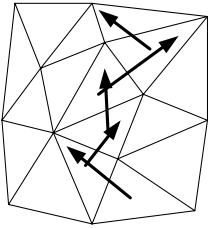
\includegraphics[scale=0.8]{images/SeparatingEdge.png}
        \caption{Переход через разделяющее ребро}
        \label{SeparatingEdge}
    \end{subfigure}
    \caption{Способы локализации вершины}
    \label{VertexLocalization}
\end{figure}
\begin{enumerate}[label=\alph*]
    \item Проводится прямая через начальный треугольник и вершину, которую требуется локализовать. Далее производятся
    переходы вдоль прямой через ребра, которые эта прямая пересекает (рис. \ref{LineThrough})
    \item На каждом шаге через центр текущего треугольника и вершину, которую требуется локализовать;
    переход осуществляется по пересеченному ребру (рис. \ref{ClosestEdge}).
    \item На каждом шаге осуществляется переход через ребро, разделяющее вершину, которую требуется локализовать, и
    вершину, которая лежит напротив этого ребра (рис. \ref{SeparatingEdge}). Данный вариант хоть и обеспечивает более
    длинный путь до цели, но он алгоритмически проще и поэтому быстрее.
\end{enumerate}

В худшем случае придется пересекать все треугольники, однако в среднем для равномерного распределения на квадрате нужно
совершить только $O(\sqrt{n})$ операций перехода\cite{Shapiro}.

\begin{figure}[H]
    \centering
    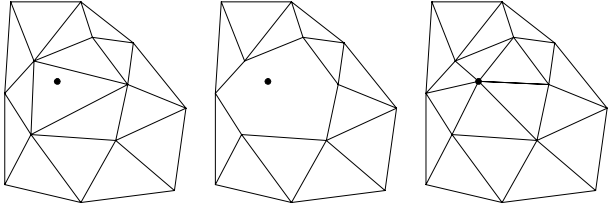
\includegraphics{images/BowyerWatson.png}
    \caption{Вставка вершины в алгоритме Бойера-Ватсона}
\end{figure}
Из известных простых итеративных алгоритмов построения триангуляции Делоне мною был выбран алгоритм Бойера-Ватсона
\cite{Bowyer, Watson}. Идея алгоритма заключается в том, что на каждом шаге удаляются все треугольники, которые
содержат вставляемую вершину, образуя при этом звездообразный многоугольник, который триангулируется, используя новую вершину.
При этом созданные треугольники не требуют перестроения, потому что новая вершина принадлежит ядру звездообразного многоугольника.
В стандартном алгоритме используется супер-структура -- геометрический объект, покрывающий все заданное множество точек,
например объемлющий прямоугольник или треугольник. В моей работе реализована процедура добавления вершины, лежащей внутри
уже построенной триангуляции (п. \ref{AddOutsideOfTriangulationVertex}).
\begin{algo}[H]
    \setstretch{1}
    \caption{Bowyer-Watson Algorithm}
    \begin{algorithmic}[1]
        \Procedure{BowyerWatson}{$points$}
            \State $triangulation \gets \{SuperStructure\}$ \Comment Супер-структура покрывающая множество точек
            \ForAll{$point \in poins$}
                \State $badTriangles \gets \{\}$
                \ForAll{$triangle \in \{triangulation\}$}
                    \If{$point \in Circumcircle(triangle)$}
                       \State $badTriangles \gets badTriangles \cup \{triangle\}$
                    \EndIf
                \EndFor
                \State $polygon \gets \{\}$
                \ForAll{$badTriangle \in badTriangles$}
                    \ForAll{$edge \in badTriangle$}
                        \If{$edge$ is not shared by any other $triangle \in badTriangles$}
                            \State $polygon \gets polygon \cup \{edge\}$
                        \EndIf
                    \EndFor
                \EndFor
                \State $triangulation \gets triangulation \setminus badTriangles$
                \ForAll{$edge \in polygon$}
                    \State $newTriangle \gets MakeTriangle(point, edge)$
                    \State $triangulation \gets triangulation \cup newTirangle$
                \EndFor
                \ForAll{$triangle \in triangulation$}
                    \If{$triangle$ contains vertex from $SuperStructure$}
                        \State $triangulation \gets triangulation \setminus triangle$
                    \EndIf
                \EndFor
            \EndFor
            \State \textbf{return} $triangulation$
        \EndProcedure
    \end{algorithmic}
\end{algo}

В данном алгоритме на первый план выходит процедура контура удаленного многоугольника, от эффективности работы которой
зависит скорость работы алгоритма.
\paragraph{Добавление вершины, лежащую вне триангуляции Делоне}
\label{AddOutsideOfTriangulationVertex}
Для того, чтобы добавить вершину, лежащую вне триангуляции, необходимо достроить треугольники до "видимой" для вершины
границы триангуляции. Назовем ребро видимым для вершины, если построенный на нем треугольник с использование вставляемой
вершины  входит в выпуклую оболочку, образуемую вершинами границы триангуляции и вставляемой вершиной.
\subsubsection{Удаление вершины из триангуляции Делоне}
\paragraph{Удаление вершины внутри триангуляции Делоне}
При удалении вершины образуется контур в виде полигона, который можно триангулировать с помощью метода отсечения
"уха" \cite{EarClipping} или алгоритма Сейдела\cite{Seidel}. Метод Ear Clipping основывается на теореме о двух "ушах" --
каждый простой полигон с количеством вершин больше 4 имеет по крайней мере 2 "уха", которые являются треугольниками с 2
сторонами, принадлежащими полигону, и 3 стороной, полностью лежащей внутри полигона. Алгоритм заключается в том, что
мы находим ухо, добавляем его в триангуляцию. Получаем новый полигон с $n - 1$ вершиной. Продолжим применять алгоритм
рекурсивно, пока $n \geq 4$. Все построенные треугольники необходимо проверить на выполнение условия Делоне и совершить
необходимые перестроения.
\paragraph{Удаление вершины на границе триангуляции Делоне}
При удалении граничной вершины необходимо удалить все треугольники, которые содержат её. Оставшаяся триангуляция может
потерять свойство выпуклости, поэтому необходимо достроить границу до выпуклой. Это можно сделать рассматриваю тройки
подряд идущих вершин границы. Если угол вогнутый, то проводится ребро. Операция выполняется до тех пор, пока не останется
ни одной тройки вершин, образующую вогнутый угол.
\section{Требования к окружению}
\begin{itemize}
    \item GPU с поддержкой OpenGL ES 2.0\textbackslash Vulkan\textbackslash Molten VK
    \item CPU с частотой 1 ГГц и выше
    \item 512 Мб RAM и больше
\end{itemize}
\subsection{Требования к программному обеспечению}
\begin{itemize}
    \item ОС Windows 8.1 и выше; macOS 10.13 и выше; дистрибутивы
    Linux, поддерживающие среду Mono; Android 5 и выше; iOS 10.3.3 и выше
    \item .NET Framework версии 4.7.1
\end{itemize}
\section{Архитектура системы}
\begin{figure}[H]
    \centering
    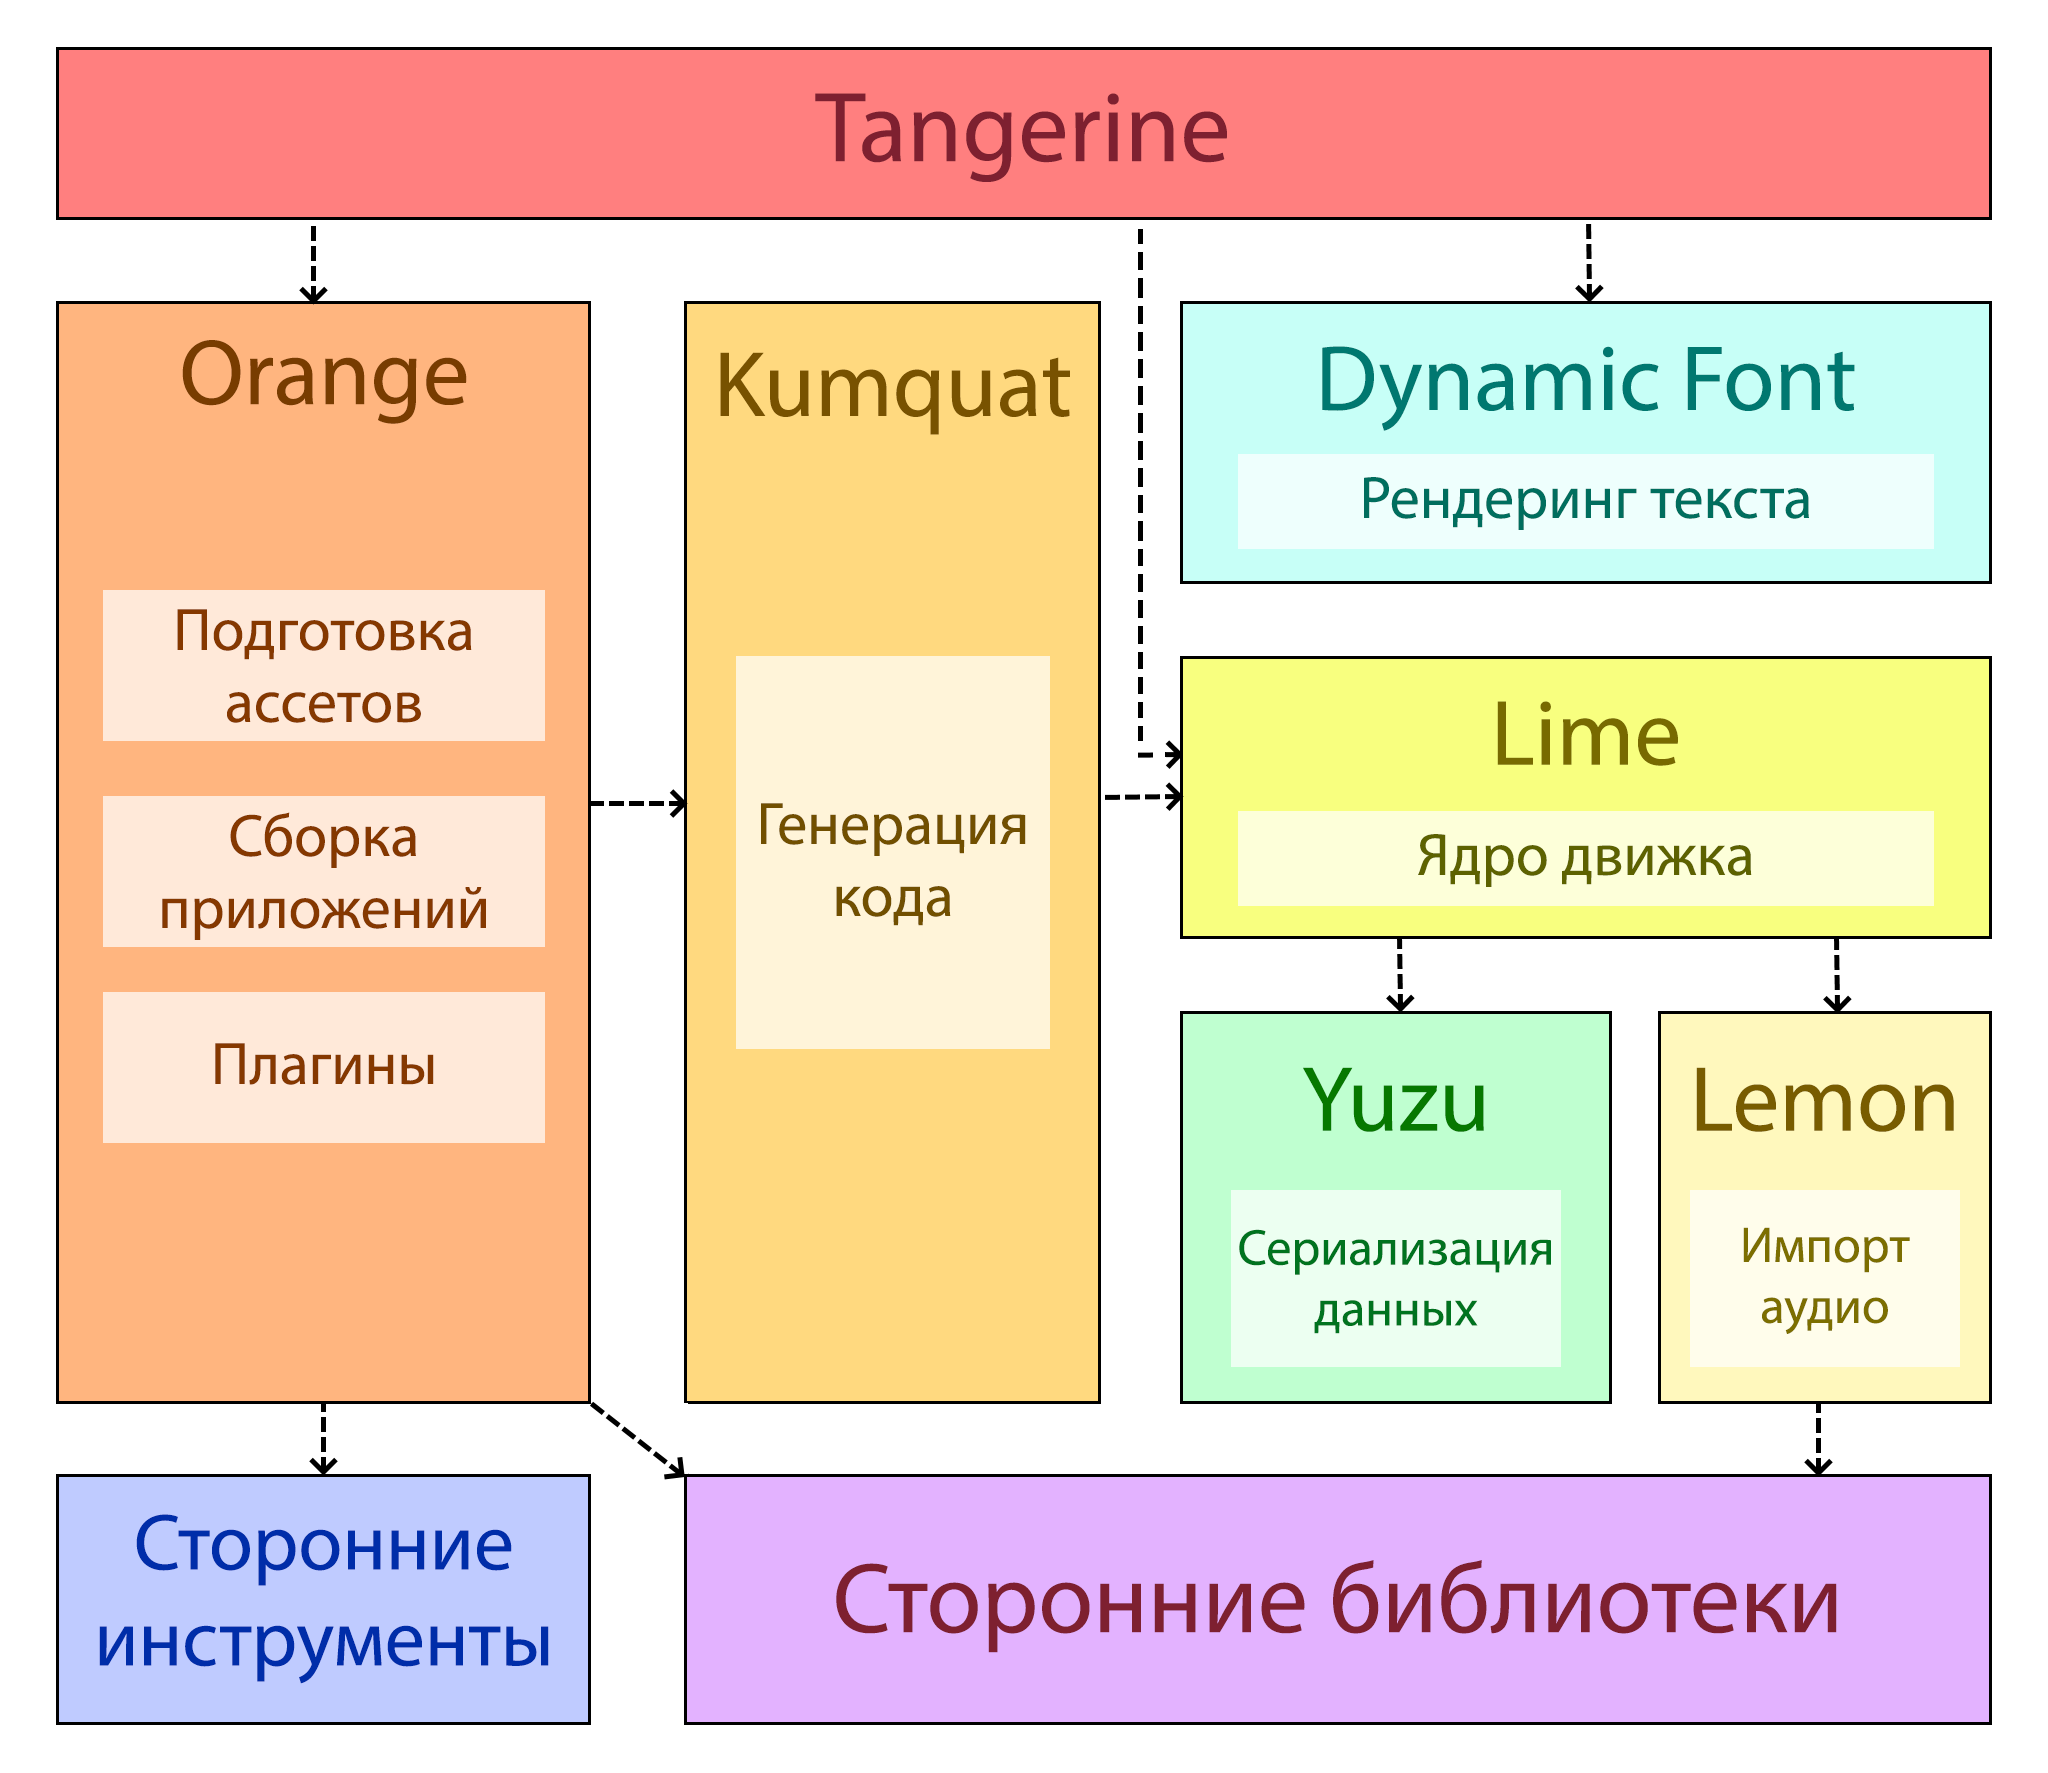
\includegraphics[scale=0.25]{images/CitrusArchitecture.png}
    \caption{Архитектура движка Citrus}
    \label{CitrusArchitecture}
\end{figure}
\subsection{Triangulator}
\begin{figure}[H]
    \centering
    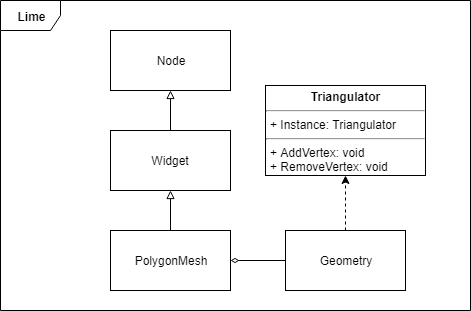
\includegraphics{images/TriangulatorArchitecture.png}
    \caption{Triangulator}
    \label{TriangulatorArchitecture}
\end{figure}
\section{Функциональные требования}
Система должна:
\begin{itemize}
    \item Редактировать структуру полигонального меша;
    \item Быть достаточно быстрой, чтобы использовать её в редакторе сцен;
    \item Быть устойчивой к ошибкам вещественной арифметики.
\end{itemize}
\section{Проект}
Методы для работы с триангуляцией представлены в синглтоне \texttt{Triangulator}. \texttt{Triangulator} используется
классом Geometry для модфикации структуры меша (данная часть описана в работе \cite{Gomenyuk}). \texttt{Triangulator}
содержит в себе следующий публичные методы:
\begin{itemize}
    \item \texttt{void AddVertex(Geometry geometry, int vertexIndex)} -- добавление вершины в триангуляцию;
    \item \texttt{void RemoveVertex(Geometry geometry, int vertexIndex)} -- удаление вершины из триангуляции.
\end{itemize}

Данные методы локализуют вершину. В зависимости от того, входит ли вершина в область триангуляции или нет, вызывается
комбинация следующих приватных методов:
\begin{itemize}
    \item \texttt{HalfEdge LocateTriangle(Geometry geometry, HalfEdge edge, int vertexIndex)} -- локализация вершины;
    \item \texttt{LinkedList<int> GetCountourPolygon(Geometry geometry, HalfEdge start, Vertex vertex)} -- выделение контура
    многоугольника, который следует удалить при вставке вершины \texttt{vertex};
    \item \texttt{LinkedList<int> GetBoundaryPolygon(Geometry geometry, HalfEdge edge)} -- выделение граничного полигона,
    образующегося при удаление вершины $edge.Origin$;
    \item \texttt{void TriangulateStarShapedPolygon(Geometry geometry, LinkedList<int> polygon, int vertexIndex)} --
    триангуляция start-shaped полигона, при условии, что вершина лежит внутри его ядра;
    \item \texttt{Queue<int> TriangulateByEarClipping(Geometry geometry, LinkedList<int> polygon)} -- триангуляция полигона
    методом "отрезания ушей";
    \item \texttt{void RestoreDelaunayProperty(Geometry geometry, Queue<int> queue)} -- проверка свойства Делоне и выполнение
    необходимых перестроений;
    \item \texttt{Queue<int> RemovePolygon(Geometry geometry, LinkedList<int> polygon)} -- удаление треугольников, входящих в
    полигон из триангуляции, с последующим достраиванием границы до выпуклой;
    \item \texttt{LinkedList<int> GetTriangulationBoundary(Geometry geometry, Vertex vertex, HalfEdge start)} -- получение
    границы триангуляции;
    \item \texttt{LinkedList<int> GetVisibleBoundary(Geometry geometry, Vertex vertex, LinkedList<int> boundary)} -- получение
    границы, видимой для вершины $vertex$;
    \item \texttt{Queue<int> TriangulateVisibleBoundary(Geometry geometry, LinkedList<int> boundary, int vertexIndex)} --
    достраивание границы триангуляции до выпуклой с учетом вершины $geometry.Vertices[vertexIndex]$.
\end{itemize}
\section{Реализация и тестирование}
Объем написанного кода 3,302 ++  959 -- (30 коммитов) в тестовом репозитории, 1200 ++, 100-- (15 коммитов) в репозитории Citrus.
Реализован виджет PolygonMesh, лишенный недостатков DistortionMesh.

Было проведено успешное ручное и автоматическое тестирование как мной, так и тестировщиками и художниками компании "Game Forest". 
По результатом тестирование работа была перенесена в рабочую копию игрового движка Citrus.
\section*{Заключение}
Во время преддипломной практики были успешно выполнены все поставленные задачи. Были успешно перенесены, дополнены и 
совмещены с остальным функционалом, представленным в \cite{Gomenyuk}, методы работы с триангуляцией множества вершин; 
проведено тестирование ;написаны отчет и документация.

При выполнении практических заданий со стороны руководителя практики была оказана значительная помощь в работе.
\newpage
\bibliographystyle{ugost2008ls}
\bibliography{references}
\end{document}
